\documentclass[11pt,a4paper,oneside]{report}

% ── Packages de base ──
\usepackage[utf8]{inputenc}
\usepackage[T1]{fontenc}
\usepackage[french]{babel}
\usepackage{pdfpages}
\usepackage{geometry}
\usepackage{fancyhdr}
\usepackage{graphicx}
\usepackage{amsmath,amsfonts,amssymb}
\usepackage{hyperref}
\usepackage{bookmark}
\usepackage{url}
\usepackage{cite}
\usepackage{setspace}
\usepackage{tocloft}
\usepackage{listings}
\usepackage[table]{xcolor}
\usepackage{colortbl}
\usepackage{float}
\usepackage{caption}
\usepackage{subcaption}
\usepackage{array}
\usepackage{longtable}
\usepackage{multirow}
\usepackage{booktabs}
\usepackage{pgfgantt}
\usepackage{tikz}
\usepackage{pdflscape}
\usepackage{titlesec}

% ── Style du rapport ──
% ── Style global du rapport UML-to-Code ──

\usepackage{placeins}
\usepackage{microtype}
\usepackage{enumitem}
\usepackage{xurl}
\usepackage{footnote}
\usepackage{etoolbox}

% Police : serif lisible (académique), pas sans-serif
\usepackage{lmodern}
\renewcommand{\familydefault}{\rmdefault}

% Espacement compact
\setstretch{1.12}
\setlength{\parskip}{0.35ex plus 0.15ex minus 0.1ex}
\setlist[itemize]{noitemsep, topsep=3pt, parsep=1pt, leftmargin=1.5em}
\setlist[enumerate]{noitemsep, topsep=3pt, parsep=1pt, leftmargin=1.8em}

% Liens et URL (coupure de ligne)
\hypersetup{
    colorlinks=true,
    linkcolor=black!80,
    filecolor=blue!70,
    urlcolor=blue!70!black,
    citecolor=black!70,
    breaklinks=true
}
\urlstyle{same}
\newcommand{\reporturl}[1]{\href{#1}{\nolinkurl{#1}}}

% Notes de bas de page
\makesavenoteenv{itemize}
\makesavenoteenv{enumerate}

% Tableaux améliorés
\newcolumntype{P}[1]{>{\raggedright\arraybackslash}p{#1}}
\newcolumntype{C}[1]{>{\centering\arraybackslash}p{#1}}
\renewcommand{\arraystretch}{1.12}
\setlength{\tabcolsep}{5pt}

\newcommand{\tablerule}{\midrule}
\newcommand{\tableheader}{\rowcolor{blue!12}\bfseries}

% En-têtes et pieds de page (référence projet en haut à droite)
\pagestyle{fancy}
\fancyhf{}
\fancyhead[L]{\small\textcolor{gray!70}{\leftmark}}
\fancyhead[R]{\small\textcolor{gray!65}{%
  Réf. : \href{https://github.com/ABAKAR5/uml-to-code}{GitHub}%
  \textbar\ \href{https://console.groq.com/docs}{Groq}%
  \textbar\ \href{https://uml-to-code-peach.vercel.app}{Vercel}%
}}
\fancyfoot[L]{\small\textcolor{gray!60}{INSTA — \annee}}
\fancyfoot[C]{\small\textbf{\thepage}}
\fancyfoot[R]{\small\textcolor{gray!60}{ABVIP}}
\renewcommand{\headrulewidth}{0.35pt}
\renewcommand{\footrulewidth}{0.25pt}
\renewcommand{\headrule}{\hbox to\headwidth{\color{blue!40}\leaders\hrule height \headrulewidth\hfill}}

% Pages préliminaires (sans en-tête gauche verbeux)
\fancypagestyle{prelim}{%
  \fancyhf{}
  \fancyfoot[C]{\small\textbf{\thepage}}
  \renewcommand{\headrulewidth}{0pt}
  \renewcommand{\footrulewidth}{0pt}
}

% Titres plus compacts
\titleformat{\chapter}[display]
  {\normalfont\huge\bfseries\color{blue!50!black}\centering}
  {\chaptertitlename\ \thechapter}
  {12pt}
  {\Huge}
\titlespacing*{\chapter}{0pt}{-18pt}{22pt}

\titleformat{\section}
  {\normalfont\Large\bfseries\color{blue!45!black}}
  {\thesection}
  {0.8em}
  {}
\titlespacing*{\section}{0pt}{10pt}{6pt}

\titleformat{\subsection}
  {\normalfont\large\bfseries}
  {\thesubsection}
  {0.6em}
  {}
\titlespacing*{\subsection}{0pt}{8pt}{4pt}

% Listings code plus compacts
\lstset{
    basicstyle=\ttfamily\footnotesize,
    aboveskip=6pt,
    belowskip=6pt
}

% Figures : légende serrée
\captionsetup{font=small, labelfont=bf, skip=6pt}

% Tableaux : taille réduite, placement souple (évite pages vides en bas)
\AtBeginEnvironment{table}{\small\centering}
\floatplacement{table}{htbp}
\floatplacement{figure}{htbp}
\raggedbottom

% TikZ (cycle de vie)
\usetikzlibrary{positioning,shapes,arrows.meta}

% Références web réutilisables (notes de bas de page + en-tête)
\newcommand{\fnGroq}{\footnote{API Groq : \reporturl{https://console.groq.com/docs}}}
\newcommand{\fnVercel}{\footnote{Frontend Vercel : \reporturl{https://uml-to-code-peach.vercel.app}}}
\newcommand{\fnRender}{\footnote{Backend Render : \reporturl{https://uml-to-code.onrender.com}}}
\newcommand{\fnGitHub}{\footnote{Dépôt GitHub : \reporturl{https://github.com/ABAKAR5/uml-to-code}}}
\newcommand{\fnStarUML}{\footnote{StarUML : \reporturl{https://staruml.io}}}
\newcommand{\fnUML}{\footnote{UML — OMG : \reporturl{https://www.omg.org/spec/UML/}}}
\newcommand{\fnReact}{\footnote{React.js : \reporturl{https://react.dev}}}
\newcommand{\fnFlask}{\footnote{Flask : \reporturl{https://flask.palletsprojects.com}}}
\newcommand{\fnMonaco}{\footnote{Monaco Editor : \reporturl{https://microsoft.github.io/monaco-editor}}}


% ── Informations du document ──
\newcommand{\titre}{Conception et réalisation d'une plateforme intelligente de conversion de diagrammes UML en code fonctionnel (UML-to-Code)}
\newcommand{\auteur}{Abakar Mahamat Brahim (ABVIP)}
\newcommand{\etablissement}{Institut National Supérieur des Sciences et Techniques d'Abéché (INSTA)}
\newcommand{\organisme}{Département de Génie Logiciel}
\newcommand{\annee}{2025-2026}
\newcommand{\encadrant}{ABOUBAKR et MAHAMAT ALHABIB}
\newcommand{\maitre}{ABOUBAKR et MAHAMAT ALHABIB}

% Titres en français (évite « Contents » / « Contenu »)
\addto\captionsfrench{%
  \renewcommand\contentsname{Table des matières}%
  \renewcommand\listfigurename{Liste des figures}%
  \renewcommand\listtablename{Liste des tableaux}%
  \renewcommand\bibname{Bibliographie}%
  \renewcommand\chaptername{Chapitre}%
}

\renewcommand{\thesection}{\arabic{section}}
\renewcommand{\thesubsection}{\thesection.\arabic{subsection}}
\renewcommand{\thesubsubsection}{\thesubsection.\arabic{subsubsection}}

\geometry{left=2.3cm,right=2cm,top=2.2cm,bottom=2.2cm,headheight=15pt}

\lstdefinelanguage{javascript}{
    keywords={break, case, catch, continue, debugger, default, delete, do, else, false, finally, for, function, if, in, instanceof, new, null, return, switch, this, throw, true, try, typeof, var, void, while, with, const, let, class, extends, export, import, super},
    morecomment=[l]{//},
    morecomment=[s]{/*}{*/},
    morestring=[b]', morestring=[b]"
}

\begin{document}

\pagenumbering{Roman}
\pagestyle{prelim}


\includepdf[pages=1]{sections/PageGarde.pdf}

\chapter*{Dédicace}
\addcontentsline{toc}{chapter}{Dédicace}
\markboth{Dédicace}{Dédicace}

\vspace*{3cm}

\begin{center}
\textit{\Large À mes parents,}\\[0.5cm]
\textit{pour leur soutien indéfectible, leurs sacrifices et leur amour inconditionnel\\
tout au long de mon parcours académique.}\\[1.5cm]

\textit{\Large À mes frères et sœurs,}\\[0.5cm]
\textit{pour leur encouragement et leur présence à chaque étape de ma vie.}\\[1.5cm]

\textit{\Large À mes enseignants de l'INSTA Abéché,}\\[0.5cm]
\textit{pour la qualité de la formation dispensée et leur dévouement\\
au service de la jeunesse tchadienne.}\\[1.5cm]

\textit{\Large À tous ceux qui croient que la technologie\\
peut transformer le continent africain.}\\[2cm]

\vspace{1cm}
\textbf{Je dédie ce travail.}
\end{center}
\chapter*{Remerciements}
\addcontentsline{toc}{chapter}{Remerciements}
\thispagestyle{plain}
\pagestyle{plain}

Je tiens à remercier tout d'abord Dieu le tout puissant pour m'avoir donné la force et la santé de mener à bien ce projet.

Mes remerciements s'adressent également à :
\begin{itemize}
    \item L'administration de l'INSTA pour le cadre d'étude.
    \item Mes enseignants du département de Génie Logiciel pour la qualité de la formation reçue.
    \item Mes encadrants, ABOUBAKR et MAHAMAT ALHABIB, pour leurs conseils précieux et leur suivi constant.
    \item Ma famille et mes amis pour leur soutien moral et matériel tout au long de mon cursus académique.
\end{itemize}

\newpage
\chapter*{Résumé}
\addcontentsline{toc}{chapter}{Résumé}
\markboth{Résumé}{Résumé}

\vspace*{0.5cm}

Ce projet présente la conception et le développement d'\textbf{UML-to-Code}, une application web full-stack permettant de transformer automatiquement des diagrammes de classes UML en code source fonctionnel, en exploitant l'Intelligence Artificielle générative \textbf{Groq Llama 3.3-70b}.

L'application accepte trois formats d'entrée : les fichiers \textbf{XMI} exportés depuis StarUML, les \textbf{images} PNG/JPG et les \textbf{documents PDF}. Elle génère du code \textbf{Python} ou \textbf{PHP} complet avec classes, attributs, méthodes et héritage, ainsi qu'un \textbf{serveur Flask} opérationnel avec routes CRUD automatiques.

L'interface web, développée avec \textbf{React.js} et le bundler Vite, intègre le \textbf{Monaco Editor} (le moteur de VS Code), un système d'historique local, un mode sombre/clair, une barre de progression en temps réel, des notifications toast et un export en archive ZIP. L'application est déployée en ligne et accessible sur \href{https://uml-to-code-peach.vercel.app}{\texttt{uml-to-code-peach.vercel.app}}.

Le projet a été réalisé selon le \textbf{modèle incrémental} en 5 incréments sur trois semaines, dans le cadre du module de Mini-Projet de Soutenance de la 3\textsuperscript{ème} année en Génie Logiciel à l'INSTA Abéché, Tchad.

\vspace{0.5cm}
\noindent\textbf{Mots-clés :} UML, génération de code, Intelligence Artificielle, LLM, Groq, Flask, React.js, MDD, Python, PHP, StarUML, XMI.

\vspace{1.5cm}

\chapter*{Abstract}
\addcontentsline{toc}{chapter}{Abstract}
\markboth{Abstract}{Abstract}

\vspace*{0.5cm}

This project presents the design and development of \textbf{UML-to-Code}, a full-stack web application that automatically transforms UML class diagrams into functional source code, leveraging the \textbf{Groq Llama 3.3-70b} generative Artificial Intelligence model.

The application accepts three input formats: \textbf{XMI} files exported from StarUML, \textbf{PNG/JPG images}, and \textbf{PDF documents}. It generates complete \textbf{Python} or \textbf{PHP} code with classes, attributes, methods and inheritance, as well as an operational \textbf{Flask server} with automatic CRUD routes.

The web interface, built with \textbf{React.js} and Vite, integrates \textbf{Monaco Editor} (the VS Code engine), a local history system, dark/light mode, a real-time progress bar, toast notifications, and ZIP archive export. The application is deployed online and accessible at \href{https://uml-to-code-peach.vercel.app}{\texttt{uml-to-code-peach.vercel.app}}.

The project was carried out using the \textbf{incremental model} in 5 increments over three weeks, as part of the Final Project module of the 3\textsuperscript{rd} year Software Engineering program at INSTA Abéché, Chad.

\vspace{0.5cm}
\noindent\textbf{Keywords:} UML, code generation, Artificial Intelligence, LLM, Groq, Flask, React.js, MDD, Python, PHP, StarUML, XMI.

\clearpage
\chapter*{Abstract}
\addcontentsline{toc}{chapter}{Abstract}
\markboth{Abstract}{Abstract}

This project presents the design and development of \textbf{UML-to-Code}, a full-stack web application that automatically transforms UML class diagrams into functional source code, leveraging the \textbf{Groq Llama 3.3-70b} generative Artificial Intelligence model\footnote{Groq documentation: \reporturl{https://console.groq.com/docs}}.

The application accepts three input formats: \textbf{XMI} files exported from StarUML, \textbf{PNG/JPG images}, and \textbf{PDF documents}. It generates complete \textbf{Python} or \textbf{PHP} code with classes, attributes, methods and inheritance, as well as an operational \textbf{Flask server} with automatic CRUD routes.

The web interface, built with \textbf{React.js} and Vite, integrates Monaco Editor, local history, themes, progress bar and ZIP export. Online deployment\footnote{\reporturl{https://uml-to-code-peach.vercel.app}}.

The project was carried out using the \textbf{incremental model} in 5 increments over three weeks, as part of the Final Project module of the 3\textsuperscript{rd} year Software Engineering program at INSTA Abéché, Chad.

\noindent\textbf{Keywords:} UML, code generation, Artificial Intelligence, LLM, Groq, Flask, React.js, MDD, Python, PHP, StarUML, XMI.

\clearpage


% ── Table des matières (page dédiée, titre en français) ──
\clearpage
\phantomsection
\addcontentsline{toc}{chapter}{Table des matières}
\chapter*{Table des matières}
\markboth{Table des matières}{Table des matières}
\makeatletter
\@starttoc{toc}
\makeatother
\thispagestyle{prelim}

\clearpage
\listoffigures
\clearpage
\listoftables
\clearpage
\chapter*{Liste des sigles et acronymes}
\addcontentsline{toc}{chapter}{Liste des sigles et acronymes}

% Définir manuellement le mark pour les en-têtes
\markboth{Liste des sigles et acronymes}{Liste des sigles et acronymes}

% Garder la numérotation romaine visible
\thispagestyle{plain}

\begin{tabular}{ll}
\textbf{API} & Application Programming Interface \\
\textbf{CIM} & Computation Independent Model \\
\textbf{CRUD} & Create, Read, Update, Delete \\
\textbf{HTTP} & Hypertext Transfer Protocol \\
\textbf{IA} & Intelligence Artificielle \\
\textbf{IDE} & Integrated Development Environment \\
\textbf{IDM} & Ingénierie Dirigée par les Modèles \\
\textbf{JSON} & JavaScript Object Notation \\
\textbf{LLM} & Large Language Model \\
\textbf{MDA} & Model-Driven Architecture \\
\textbf{MDD} & Model-Driven Development \\
\textbf{MOF} & Meta Object Facility \\
\textbf{OMG} & Object Management Group \\
\textbf{PFE} & Projet de Fin d'Études \\
\textbf{PHP} & PHP: Hypertext Preprocessor \\
\textbf{PIM} & Platform Independent Model \\
\textbf{PSM} & Platform Specific Model \\
\textbf{REST} & Representational State Transfer \\
\textbf{UML} & Unified Modeling Language \\
\textbf{XMI} & XML Metadata Interchange \\
\textbf{XML} & eXtensible Markup Language \\
\end{tabular}

\newpage


\clearpage
\pagenumbering{arabic}
\pagestyle{fancy}

\chapter*{Introduction Générale}
\addcontentsline{toc}{chapter}{Introduction Générale}
\thispagestyle{plain}
\pagestyle{plain}
\markboth{}{}

Le domaine de l'ingénierie logicielle est en constante évolution, cherchant sans cesse à optimiser les processus de développement pour réduire les délais de livraison tout en maintenant un haut niveau de qualité. Dans le cycle de vie classique du développement logiciel, la phase de conception, souvent modélisée à l'aide du langage UML (Unified Modeling Language), est une étape fondamentale. Elle permet d'établir une architecture claire et de définir les interactions entre les différentes composantes du système avant même d'écrire la première ligne de code.

Cependant, la traduction de ces modèles conceptuels en code source concret reste une tâche laborieuse, répétitive et chronophage. Bien que l'architecture soit définie, le développeur doit manuellement recréer les classes, les attributs, les méthodes et les relations dans le langage cible. Cette étape manuelle est non seulement une perte de temps précieux, mais elle est également sujette à des erreurs humaines qui peuvent introduire des incohérences entre le modèle conçu et l'implémentation finale.

C'est dans ce contexte que s'inscrit notre projet de fin de cycle intitulé \textbf{UML-to-Code}. Ce projet a pour ambition d'automatiser cette transition délicate entre la conception et l'implémentation. \textbf{UML-to-Code} est une plateforme web intelligente conçue pour transformer automatiquement des diagrammes de classes UML en code source fonctionnel, structuré et prêt à l'emploi. 

Notre solution se démarque par une approche hybride innovante :
\begin{itemize}
    \item \textbf{Une approche algorithmique déterministe} : capable d'analyser des fichiers XMI (XML Metadata Interchange) exportés depuis des outils de modélisation standards comme StarUML.
    \item \textbf{Une approche basée sur l'Intelligence Artificielle} : intégrant un modèle de langage avancé (LLM - Llama 3.3 via Groq) pour analyser des diagrammes sous format image (PNG, JPG) ou PDF, offrant ainsi une flexibilité sans précédent aux développeurs qui préfèrent dessiner leurs architectures.
\end{itemize}

Ce rapport s'attache à décrire de manière exhaustive les différentes phases qui ont jalonné la réalisation de cette plateforme. Le document est structuré de la manière suivante :

\begin{itemize}
    \item Le \textbf{Chapitre 1} dresse le contexte du projet, l'étude de l'existant, ainsi que l'analyse détaillée des besoins fonctionnels et non fonctionnels auxquels l'application doit répondre.
    \item Le \textbf{Chapitre 2} est consacré à la conception de la solution. Il y est abordé l'approche théorique (MDA/MDD), l'architecture logicielle retenue et les différents diagrammes modélisant le comportement du système.
    \item Le \textbf{Chapitre 3} détaille la phase de réalisation et d'implémentation. Nous y présenterons le cycle de vie adopté, les choix technologiques (React, Flask, Groq), ainsi que des extraits de code illustrant les mécanismes clés comme le parsing XML.
\end{itemize}

Enfin, une \textbf{Conclusion Générale} viendra synthétiser les résultats obtenus, les compétences acquises au cours de ce projet et les perspectives d'évolution envisageables pour la plateforme UML-to-Code.

\newpage

\chapter{Étude Préliminaire et Analyse des Besoins}

\section*{Introduction}
\addcontentsline{toc}{section}{Introduction}

Dans ce premier chapitre, nous présentons l'Institut National Supérieur des Sciences et Techniques d'Abéché (INSTA), notre établissement de formation. Nous exposons ensuite le contexte général du projet, l'analyse de l'existant, la problématique identifiée, ainsi que les besoins fonctionnels et non fonctionnels du système à concevoir.

%=============================================
\section{Contexte Institutionnel : l'INSTA}
%=============================================

\subsection{Présentation générale}

L'Institut National Supérieur des Sciences et Techniques d'Abéché (INSTA) est un établissement public d'enseignement supérieur à caractère scientifique et technique, situé dans la ville d'Abéché (province du Ouaddaï), au Nord-Est du Tchad. Créé initialement sous le nom d'Institut Universitaire des Sciences et Techniques d'Abéché (IUSTA) en 1997, il a été rebaptisé INSTA par l'Ordonnance N°004/PR/MES/2015 du 02 mars 2015.

\subsection{Missions de l'INSTA}

L'institut poursuit plusieurs missions fondamentales :

\begin{itemize}
    \item \textbf{Formation académique et professionnelle} : former des étudiants dans divers domaines techniques et scientifiques, en vue de répondre aux besoins du marché de l'emploi.
    \item \textbf{Recherche et innovation} : promouvoir la recherche scientifique et valoriser les résultats pour répondre aux besoins du pays.
    \item \textbf{Partenariats} : établir des collaborations avec des institutions nationales et internationales pour renforcer la qualité de l'enseignement.
    \item \textbf{Contribution au développement} : fournir au marché de l'emploi des ingénieurs compétents capables d'apporter des solutions aux problématiques locales.
\end{itemize}

\subsection{Offres de formation}

L'INSTA offre deux cycles principaux :

\begin{itemize}
    \item \textbf{Premier cycle} : Licence professionnelle (3 ans) formant des licenciés professionnels dans les domaines scientifiques et techniques.
    \item \textbf{Deuxième cycle} : Master (2 ans), divisé en Master professionnel et recherche, dans les domaines de Génie Électrique, Génie Mécanique, Génie Énergétique, Sciences Biomédicales et Sciences et Techniques d'Élevage.
\end{itemize}

\subsection{Départements de l'INSTA}

L'institut est composé de plusieurs départements :

\begin{itemize}
    \item Département de Génie Informatique (GI) — option Génie Logiciel
    \item Département de Génie Mécanique (GM)
    \item Département de Génie Électrique (GE)
    \item Département de Génie Énergétique (GEN)
    \item Département de Télécommunication et Réseau (TLC)
    \item Département Conception, Installation et Maintenance des Systèmes (CIMS)
    \item Département des Sciences et Techniques d'Élevage (STE)
    \item Département des Sciences Biomédicales et Pharmaceutiques (SBMP)
\end{itemize}

%=============================================
\section{Contexte Général du Projet}
%=============================================

\subsection{Le Génie Logiciel et la modélisation UML}

Le Génie Logiciel est la discipline qui s'intéresse à la conception, au développement, à la maintenance et à la gestion de systèmes logiciels de qualité. Parmi les pratiques fondamentales de cette discipline, la modélisation occupe une place centrale. Elle permet de représenter un système sous forme abstraite avant son implémentation, facilitant ainsi la communication entre les parties prenantes et la détection précoce des erreurs de conception.

L'UML (\textit{Unified Modeling Language}) est le langage de modélisation le plus utilisé dans l'industrie du logiciel. Il propose un ensemble de diagrammes standardisés permettant de décrire l'architecture statique et dynamique d'un système logiciel. Pour notre projet, nous avons utilisé trois types de diagrammes :

\begin{table}[htbp]
\centering
\renewcommand{\arraystretch}{1.4}
\begin{tabular}{|l|p{5cm}|l|}
\hline
\rowcolor{gray!30}
\textbf{Diagramme} & \textbf{Objectif} & \textbf{Type} \\
\hline
Diagramme de classes & Représenter la structure statique du système : classes, attributs, méthodes et relations & Statique \\
\hline
Diagramme de cas d'utilisation & Décrire les interactions entre les acteurs et le système & Fonctionnel \\
\hline
Diagramme de séquence & Illustrer les échanges entre composants dans un ordre temporel & Dynamique \\
\hline
\end{tabular}
\caption{Diagrammes UML utilisés dans le projet}
\end{table}

\subsection{Le Développement Dirigé par les Modèles (MDD)}

Le \textbf{Développement Dirigé par les Modèles} (MDD — \textit{Model-Driven Development}) est un paradigme de développement logiciel qui place le modèle au cœur du processus de développement. L'idée fondatrice du MDD est que le modèle n'est plus un simple document de documentation, mais un artefact de première classe à partir duquel le code source peut être généré automatiquement.

Dans ce paradigme, on distingue :
\begin{itemize}
    \item Le \textbf{PIM} (\textit{Platform Independent Model}) : le modèle UML indépendant de toute plateforme
    \item Le \textbf{PSM} (\textit{Platform Specific Model}) : le code source généré pour une plateforme cible (Python, PHP, etc.)
    \item La \textbf{transformation} : le processus automatique qui convertit le PIM en PSM
\end{itemize}

Notre projet s'inscrit exactement dans cette approche : le diagramme UML est le PIM, et le code Python ou PHP généré est le PSM.

\subsection{L'Intelligence Artificielle générative}

L'avènement des \textbf{Grands Modèles de Langage} (LLM — \textit{Large Language Models}) représente une révolution dans le domaine de l'Intelligence Artificielle. Ces modèles, entraînés sur des milliards de lignes de texte et de code source, sont capables de comprendre et de générer du code source de manière contextuelle et cohérente.

Dans le cadre de ce projet, nous exploitons le modèle \textbf{Groq Llama 3.3-70b}, un LLM open source de 70 milliards de paramètres développé par Meta et hébergé sur l'infrastructure d'inférence ultra-rapide \textbf{Groq}, qui permet des temps de génération de l'ordre de 2 à 5 secondes.

\subsection{Le format XMI}

Le format \textbf{XMI} (\textit{XML Metadata Interchange}) est un standard défini par l'OMG\footnote{Object Management Group : \reporturl{https://www.omg.org}} pour l'échange de modèles UML entre différents outils de modélisation. C'est un fichier texte structuré en XML qui contient la description complète d'un modèle UML : classes, attributs, méthodes, relations et héritage.

StarUML\fnStarUML, l'outil de modélisation que nous utilisons, permet d'exporter les diagrammes de classes au format XMI 2.1. Notre application parse ce fichier pour en extraire automatiquement la structure orientée objet et générer le code correspondant.

%=============================================
\section{Analyse de l'Existant}
%=============================================

\subsection{Outils existants de transformation UML vers code}

Plusieurs outils de transformation UML vers code existent sur le marché. Nous en avons analysé les principaux afin d'identifier leurs limites :

\begin{table}[htbp]
\centering
\renewcommand{\arraystretch}{1.4}
\begin{tabular}{|l|l|l|p{4.5cm}|}
\hline
\rowcolor{gray!30}
\textbf{Outil} & \textbf{Langages générés} & \textbf{Format entrée} & \textbf{Limites principales} \\
\hline
Acceleo (Eclipse) & Java, Python, PHP & XMI/EMF & Très complexe, lourd à installer \\
\hline
AndroMDA & Java EE uniquement & XMI & Limité à Java, pas d'IA \\
\hline
GenMyModel & Java, Python & En ligne & Payant, pas open source \\
\hline
StarUML Plugins & JavaScript, Java & .mdj & Limité, pas d'IA générative \\
\hline
Solutions manuelles & Tous langages & Tous formats & Lent, source d'erreurs \\
\hline
\end{tabular}
\caption{Comparatif des outils existants de transformation UML vers code}
\end{table}

\subsection{Limites des solutions existantes}

L'analyse comparative révèle plusieurs lacunes communes :

\begin{itemize}
    \item \textbf{Complexité d'installation} : des outils comme Acceleo nécessitent une installation lourde et une configuration complexe
    \item \textbf{Absence d'IA} : aucun outil n'intègre de modèle d'IA générative pour produire un code contextuel
    \item \textbf{Formats d'entrée limités} : la plupart n'acceptent que le format XMI, excluant les images et les PDF
    \item \textbf{Coût} : certaines solutions performantes sont payantes et propriétaires
    \item \textbf{Pas de génération de serveur} : aucun outil ne génère automatiquement un serveur REST opérationnel
\end{itemize}

\subsection{Valeur ajoutée de notre solution}

Face à ces limitations, \textbf{UML-to-Code} apporte une réponse innovante :
\begin{itemize}
    \item Intégration d'une IA générative (\textbf{Groq Llama 3.3-70b}) pour un code contextuel et complet
    \item Support de plusieurs formats d'entrée : XMI, image PNG/JPG, PDF
    \item Génération automatique d'un serveur Flask complet avec routes CRUD
    \item Interface web moderne avec Monaco Editor, historique local, mode sombre/clair
    \item Export en archive ZIP du projet complet prêt à déployer
    \item Déploiement en ligne accessible via Vercel\fnVercel{} et Render\fnRender
    \item Solution légère, open source et sans installation complexe
\end{itemize}

%=============================================
\section{Spécification des Besoins}
%=============================================

\subsection{Acteurs du système}

\begin{table}[htbp]
\centering
\renewcommand{\arraystretch}{1.4}
\begin{tabular}{|l|p{4cm}|p{6cm}|}
\hline
\rowcolor{gray!30}
\textbf{Acteur} & \textbf{Rôle} & \textbf{Interactions principales} \\
\hline
\textbf{Utilisateur} & Étudiant ou développeur utilisant l'outil & Upload fichier, choix options, génération, visualisation Monaco Editor, copie, téléchargement, consultation historique \\
\hline
\textbf{API Groq (IA)} & Modèle Llama 3.3-70b & Reçoit la description UML extraite, retourne le code généré \\
\hline
\textbf{Backend Flask} & Serveur Python & Orchestration, parsing XMI/image/PDF, appel API Groq, génération ZIP \\
\hline
\textbf{localStorage} & Stockage navigateur & Persiste l'historique des 10 dernières générations et le thème \\
\hline
\end{tabular}
\caption{Acteurs du système UML-to-Code}
\end{table}

\subsection{Exigences Fonctionnelles}

Les exigences fonctionnelles sont regroupées par module dans le tableau~\ref{tab:ef-complet}. Les priorités \og Haute \fg{} et \og Moyenne \fg{} guident l'ordre de réalisation des incréments.

\begin{longtable}{|c|l|P{6.8cm}|c|}
\hline
\rowcolor{blue!12}
\textbf{ID} & \textbf{Module} & \textbf{Exigence} & \textbf{Priorité} \\
\hline
\endfirsthead
\hline
\rowcolor{blue!12}
\textbf{ID} & \textbf{Module} & \textbf{Exigence} & \textbf{Priorité} \\
\hline
\endhead
EF-01 & Upload & Accepter les fichiers XMI exportés depuis StarUML\fnStarUML & Haute \\
\hline
EF-02 & Upload & Accepter les images PNG et JPG de diagrammes UML & Haute \\
\hline
EF-03 & Upload & Accepter les fichiers PDF contenant un diagramme UML & Moyenne \\
\hline
EF-04 & Upload & Valider le format du fichier avant traitement & Haute \\
\hline
EF-05 & Upload & Afficher un message d'erreur en cas de format invalide & Haute \\
\hline
EF-06 & Upload & Afficher un aperçu visuel du diagramme pour PNG/JPG & Moyenne \\
\hline
EF-07 & Parsing & Parser les classes, attributs et méthodes depuis un XMI & Haute \\
\hline
EF-08 & Parsing & Extraire les relations d'héritage entre classes & Haute \\
\hline
EF-09 & Parsing & Extraire les associations et agrégations & Moyenne \\
\hline
EF-10 & Parsing & Envoyer l'image/PDF à Groq (vision IA)\fnGroq & Haute \\
\hline
EF-11 & Génération & Appeler l'API Groq (Llama 3.3-70b) avec la description UML & Haute \\
\hline
EF-12 & Génération & Générer le code Python (\texttt{\_\_init\_\_}, getters, setters) & Haute \\
\hline
EF-13 & Génération & Générer le code PHP (constructeur, getters) & Haute \\
\hline
EF-14 & Génération & Générer un serveur Flask avec routes CRUD\fnFlask & Haute \\
\hline
EF-15 & Génération & Choix du langage : Python ou PHP & Haute \\
\hline
EF-16 & Génération & Choix du mode : Algorithmique ou IA Groq & Haute \\
\hline
EF-17 & Interface & Afficher le code dans Monaco Editor\fnMonaco & Haute \\
\hline
EF-18 & Interface & Onglets Code et Serveur Flask séparés & Haute \\
\hline
EF-19 & Interface & Copie du code en un clic & Haute \\
\hline
EF-20 & Interface & Téléchargement du fichier \texttt{.py} ou \texttt{.php} & Haute \\
\hline
EF-21 & Interface & Export en archive ZIP & Haute \\
\hline
EF-22 & Interface & Barre de progression en temps réel & Haute \\
\hline
EF-23 & Interface & Historique local (10 générations) & Haute \\
\hline
EF-24 & Interface & Mode sombre / mode clair & Moyenne \\
\hline
EF-25 & Interface & Notifications toast & Moyenne \\
\hline
\caption{Exigences fonctionnelles complètes du système UML-to-Code}
\label{tab:ef-complet}
\end{longtable}

\subsection{Exigences Non Fonctionnelles}

\begin{table}[htbp]
\centering
\renewcommand{\arraystretch}{1.15}
\begin{tabular}{|l|P{4.8cm}|P{4.2cm}|}
\hline
\rowcolor{blue!12}
\textbf{Catégorie} & \textbf{Exigence} & \textbf{Critère mesurable} \\
\hline
Performance & Temps de réponse de la génération & $<$ 15 secondes par diagramme \\
\hline
Disponibilité & Application accessible en ligne\fnVercel & 24h/24 via Vercel \\
\hline
Fiabilité & Taux de succès de la génération & $>$ 90\% sur les cas de test \\
\hline
Maintenabilité & Code source documenté et structuré & Commentaires sur chaque fonction \\
\hline
Portabilité & Fonctionne sur Windows et Linux & Testé sur les deux systèmes \\
\hline
Sécurité & Clé API en variable d'environnement & Fichier \texttt{.env} non versionné \\
\hline
Utilisabilité & Interface intuitive sans formation & Prise en main $<$ 5 minutes \\
\hline
Responsivité & Interface adaptée mobile et desktop & 320px à 1440px \\
\hline
\end{tabular}
\caption{Exigences non fonctionnelles}
\label{tab:enf}
\end{table}

\section*{Conclusion}
\addcontentsline{toc}{section}{Conclusion}

Dans ce premier chapitre, nous avons présenté l'établissement d'accueil INSTA et exposé le contexte général du projet. Nous avons analysé les solutions existantes de transformation UML vers code et identifié leurs limites, ce qui nous a permis de justifier la valeur ajoutée de notre solution UML-to-Code\fnGitHub. Enfin, nous avons spécifié les besoins fonctionnels et non fonctionnels du système à concevoir. Le chapitre suivant sera consacré à la conception et la modélisation du système.
\chapter{Conception de la Solution}

\section{Approche Théorique : L'Ingénierie Dirigée par les Modèles}

La conception de notre solution repose sur un socle théorique solide largement reconnu dans le domaine du génie logiciel : l'Ingénierie Dirigée par les Modèles (IDM). 

\subsection{Le concept du MDD (Model-Driven Development)}
Notre projet s'inscrit pleinement dans l'approche \textbf{MDD (Model-Driven Development)}. Dans cette méthodologie, le modèle n'est plus considéré comme un simple document de documentation ou un croquis préliminaire, mais comme l'artefact principal et central du processus de développement. L'objectif est de générer tout ou partie du code source du système directement à partir de ce modèle. Cette automatisation garantit que l'implémentation reflète fidèlement la conception, réduisant ainsi la fracture entre l'architecte et le développeur.

\subsection{L'Architecture MDA (Model-Driven Architecture)}
Pour concrétiser le MDD, nous nous appuyons sur la \textbf{MDA (Model-Driven Architecture)}, un cadre conceptuel standardisé par l'OMG. La MDA prône la séparation stricte entre les spécifications fonctionnelles d'un système et son implémentation technologique. Elle distingue trois niveaux d'abstraction majeurs :

\begin{itemize}
    \item \textbf{CIM (Computation Independent Model)} : Le modèle indépendant des calculs. Il représente la vue métier du système, les exigences des utilisateurs, sans aucune considération technologique.
    \item \textbf{PIM (Platform Independent Model)} : Le modèle indépendant de la plateforme. Il décrit la structure et le comportement du système (dans notre cas, le diagramme de classes UML fourni en entrée par l'utilisateur).
    \item \textbf{PSM (Platform Specific Model)} : Le modèle spécifique à la plateforme. Il représente le code source ciblé (Python, PHP, ou Flask) généré par notre application.
\end{itemize}

L'application \textbf{UML-to-Code} agit donc comme le moteur de transformation automatisé (Transformation Engine) permettant de passer du niveau \textbf{PIM} au niveau \textbf{PSM}.

\section{Stratégies de Transformation}
Pour réaliser cette transformation PIM vers PSM, notre plateforme innove en proposant deux approches distinctes et complémentaires.

\subsection{L'Approche Algorithmique (Déterministe)}
Cette méthode est basée sur des règles de transformation strictes et codées en dur. Le système parcourt le fichier XMI et applique des équivalences :
\begin{itemize}
    \item Un nœud \texttt{uml:Class} déclenche la création d'une structure \texttt{class NomClasse:} en Python.
    \item Un nœud \texttt{ownedAttribute} avec \texttt{visibility="private"} génère des variables encapsulées (\texttt{\_\_attribut} en Python).
\end{itemize}
\textit{Avantages :} Cette approche est extrêmement rapide, fiable, ne nécessite aucune connexion internet, et donne un résultat 100\% prédictible.

\subsection{L'Approche par IA Générative (LLM)}
Pour contourner les limites du parsing algorithmique (qui exige un fichier XMI parfaitement formaté), nous intégrons une approche sémantique. Le modèle XMI, ou directement une capture d'écran du diagramme, est envoyé à un Large Language Model (Llama 3.3 via l'API Groq) accompagné d'un prompt métier très précis. L'IA analyse visuellement ou textuellement les entités et génère le code.
\textit{Avantages :} Une flexibilité immense permettant de comprendre des croquis à main levée, des PDF, et de générer du code métier complexe.

\section{Architecture Globale du Système}
Pour supporter ces deux approches, nous avons opté pour une architecture logicielle moderne, séparant clairement les responsabilités.

\subsection{Architecture Client-Serveur}
Le système est divisé en trois tiers principaux :
\begin{itemize}
    \item \textbf{Le Frontend (Client)} : Développé en React.js avec le bundler Vite. Il offre une interface riche ("Single Page Application"), gère les interactions utilisateur, la prévisualisation des fichiers et intègre un éditeur de code avancé (Monaco Editor).
    \item \textbf{Le Backend (Serveur API)} : Développé en Python avec le micro-framework Flask. Il reçoit les fichiers du frontend, orchestre le parsing XML, exécute les algorithmes de génération, prépare les fichiers ZIP, et gère la communication avec les services externes.
    \item \textbf{Le Service IA Externe} : L'API cloud de Groq qui exécute le modèle open-source Llama 3.3 pour les tâches de vision et de génération de texte.
\end{itemize}

\section{Modélisation UML de la Solution}

\subsection{Diagramme de Cas d'Utilisation}
Les acteurs interagissant avec le système sont le \textbf{Développeur} (utilisateur final) et le \textbf{Système Externe} (API Groq).
Les cas d'utilisation principaux pour le développeur incluent :
\begin{itemize}
    \item Uploader un modèle (XMI, PNG, PDF).
    \item Configurer la génération (choix du langage et du mode).
    \item Lancer la génération de code.
    \item Consulter l'historique des générations.
    \item Exporter le projet généré (Format texte ou ZIP).
\end{itemize}

\subsection{Diagramme de Séquence (Génération via IA)}
Afin de comprendre la cinématique d'une requête complexe, voici les étapes d'une génération utilisant l'IA :
\begin{enumerate}
    \item \textbf{Développeur} $\rightarrow$ \textbf{Frontend} : Soumet une image de diagramme et sélectionne "Génération Python via IA".
    \item \textbf{Frontend} $\rightarrow$ \textbf{Backend Flask} : Envoi d'une requête POST contenant l'image et les paramètres.
    \item \textbf{Backend Flask} $\rightarrow$ \textbf{API Groq} : Formation d'un prompt d'instruction couplé à l'image encodée en base64. L'appel réseau est initié.
    \item \textbf{API Groq} $\rightarrow$ \textbf{Backend Flask} : Après un traitement d'environ 10 à 15 secondes, l'IA retourne le code généré sous forme de texte brut.
    \item \textbf{Backend Flask} $\rightarrow$ \textbf{Frontend} : Le texte est formaté, encapsulé dans un objet JSON, et renvoyé au client.
    \item \textbf{Frontend} $\rightarrow$ \textbf{Développeur} : Affichage du code dans le Monaco Editor avec coloration syntaxique.
\end{enumerate}

\section{Conclusion du chapitre}
L'architecture conçue pour UML-to-Code repose sur les principes de la MDA, traduits par une implémentation client-serveur moderne. La dualité algorithme/IA permet de couvrir un spectre très large de cas d'usage, allant de l'export d'entreprise strict à l'esquisse rapide. Le chapitre suivant s'attachera à détailler les choix techniques et la réalisation concrète de cette conception.
\chapter{Réalisation et Implémentation}

\section{Environnement de Développement}

\subsection{Matériel et système d'exploitation}

Le développement du projet a été réalisé sur la configuration suivante :

\begin{table}[H]
\centering
\renewcommand{\arraystretch}{1.4}
\begin{tabular}{|l|l|}
\hline
\rowcolor{gray!30}
\textbf{Composant} & \textbf{Détail} \\
\hline
Machine & HP (ordinateur portable) \\
\hline
Système d'exploitation & Windows 11 \\
\hline
Éditeur de code & Visual Studio Code \\
\hline
Terminal & PowerShell / Git Bash \\
\hline
Versioning & Git + GitHub (\href{https://github.com/ABAKAR5/uml-to-code}{github.com/ABAKAR5/uml-to-code}) \\
\hline
Modélisation UML & StarUML \\
\hline
\end{tabular}
\caption{Environnement matériel et logiciel de développement}
\end{table}

\subsection{Outils et technologies utilisés}

\subsubsection{Backend — Python Flask}

Le backend a été développé en \textbf{Python} avec le micro-framework \textbf{Flask 3.0.0}. L'environnement virtuel Python a été utilisé pour isoler les dépendances du projet. Les principales bibliothèques utilisées sont :

\begin{itemize}
    \item \textbf{Flask} : serveur web et gestion des routes API REST
    \item \textbf{flask-cors} : gestion des requêtes Cross-Origin (CORS) depuis le frontend React
    \item \textbf{groq} : client officiel Python pour l'API Groq
    \item \textbf{PyMuPDF (fitz)} : conversion des fichiers PDF en images pour l'analyse visuelle
    \item \textbf{python-dotenv} : chargement des variables d'environnement depuis le fichier \texttt{.env}
    \item \textbf{zipfile} : module natif Python pour la création des archives ZIP
    \item \textbf{xml.etree.ElementTree} : module natif Python pour le parsing des fichiers XMI
\end{itemize}

\subsubsection{Frontend — React + Vite}

L'interface utilisateur a été développée avec \textbf{React.js} et le bundler \textbf{Vite 6.x}. Les principales bibliothèques utilisées sont :

\begin{itemize}
    \item \textbf{@monaco-editor/react} : intégration de Monaco Editor (le moteur de VS Code)
    \item \textbf{axios} : client HTTP pour les requêtes vers le backend Flask
    \item \textbf{react-icons} : bibliothèque d'icônes (FaHome, FaBolt, FaRobot, etc.)
    \item \textbf{CSS Variables} : système de thèmes (sombre/clair) via variables CSS natives
\end{itemize}

\section{Implémentation du Backend}

\subsection{Structure du Backend}

Le backend Flask est organisé de manière modulaire, chaque module ayant une responsabilité précise :

\begin{table}[H]
\centering
\renewcommand{\arraystretch}{1.4}
\begin{tabular}{|l|p{8cm}|}
\hline
\rowcolor{gray!30}
\textbf{Fichier} & \textbf{Rôle} \\
\hline
\texttt{app.py} & Point d'entrée du serveur Flask, configuration CORS \\
\hline
\texttt{routes/upload.py} & Endpoints API : \texttt{/api/upload} et \texttt{/api/download-zip} \\
\hline
\texttt{parser/xmi\_parser.py} & Parsing des fichiers XMI et extraction des classes UML \\
\hline
\texttt{parser/image\_parser.py} & Préparation des images et PDF pour l'analyse IA \\
\hline
\texttt{ai/gemma\_client.py} & Client API Groq (Llama 3.3-70b) \\
\hline
\texttt{generator/base\_generator.py} & Classe abstraite de génération de code \\
\hline
\texttt{generator/python\_generator.py} & Générateur de code Python \\
\hline
\texttt{generator/php\_generator.py} & Générateur de code PHP \\
\hline
\texttt{generator/server\_generator.py} & Générateur du serveur Flask automatique \\
\hline
\texttt{generator/zip\_generator.py} & Création de l'archive ZIP du projet \\
\hline
\end{tabular}
\caption{Structure modulaire du backend Flask}
\end{table}

\subsection{Parser XMI}

Le parser XMI est le composant algorithmique central du backend. Il analyse les fichiers XMI exportés depuis StarUML et en extrait la structure orientée objet.

Le fichier XMI est un format XML standardisé par l'OMG (\textit{Object Management Group}) pour l'échange de modèles UML. Voici un exemple de fichier XMI d'entrée :

\begin{lstlisting}[language=XML, caption=Exemple de fichier XMI d'entrée]
<packagedElement xmi:type="uml:Class" name="Etudiant">
  <ownedAttribute name="nom" visibility="private"
                  xmi:type="uml:Property">
    <type xmi:type="uml:PrimitiveType" href="String"/>
  </ownedAttribute>
  <ownedOperation name="getNom" visibility="public"
                  xmi:type="uml:Operation"/>
</packagedElement>
\end{lstlisting}

À partir de ce fichier, le parser extrait :
\begin{itemize}
    \item Le nom de la classe : \texttt{Etudiant}
    \item L'attribut privé : \texttt{nom: String}
    \item La méthode publique : \texttt{getNom(): String}
\end{itemize}

\subsection{Génération de Code Python}

Le \texttt{PythonGenerator} hérite de \texttt{BaseGenerator} et implémente la génération de classes Python complètes. Voici un exemple de code Python généré à partir du diagramme XMI :

\begin{lstlisting}[language=Python, caption=Exemple de code Python généré]
class Etudiant:
    """Etudiant class"""
    def __init__(self):
        self.__nom = ""
        self.__age = 0

    def get_nom(self):
        return self.__nom

    def set_nom(self, nom):
        self.__nom = nom

    def get_age(self):
        return self.__age

    def set_age(self, age):
        self.__age = age
\end{lstlisting}

\subsection{Génération de Code PHP}

Le \texttt{PHPGenerator} génère des classes PHP 8+ avec gestion de la visibilité, constructeur et getters/setters :

\begin{lstlisting}[language=PHP, caption=Exemple de code PHP généré]
<?php
class Etudiant {
    private $nom;
    private $age;

    public function __construct() {
        $this->nom = "";
        $this->age = 0;
    }

    public function getNom() {
        return $this->nom;
    }

    public function setNom($nom) {
        $this->nom = $nom;
    }
}
?>
\end{lstlisting}

\subsection{Génération du Serveur Flask}

Le \texttt{FlaskServerGenerator} génère automatiquement un serveur Flask complet avec les routes CRUD pour chaque classe détectée :

\begin{lstlisting}[language=Python, caption=Exemple de serveur Flask généré]
from flask import Flask, jsonify, request
app = Flask(__name__)

etudiant_store = []

@app.route('/etudiants', methods=['GET'])
def get_etudiants():
    return jsonify(etudiant_store)

@app.route('/etudiants', methods=['POST'])
def create_etudiant():
    data = request.json
    etudiant_store.append(data)
    return jsonify(data), 201

@app.route('/etudiants/<int:id>', methods=['PUT'])
def update_etudiant(id):
    data = request.json
    etudiant_store[id] = data
    return jsonify(data)

@app.route('/etudiants/<int:id>', methods=['DELETE'])
def delete_etudiant(id):
    etudiant_store.pop(id)
    return jsonify({'message': 'Deleted'})

if __name__ == '__main__':
    app.run(debug=True)
\end{lstlisting}

\section{Implémentation du Frontend}

\subsection{Structure du Frontend}

L'interface utilisateur est une Single Page Application (SPA) développée avec React.js. Elle est organisée en une seule page composée de plusieurs sections :

\begin{itemize}
    \item \textbf{Navbar} : navigation responsive avec menu hamburger mobile et bascule de thème
    \item \textbf{Hero} : section d'accueil avec présentation et aperçu du code généré
    \item \textbf{Features} : présentation des fonctionnalités clés
    \item \textbf{How it works} : workflow en 4 étapes
    \item \textbf{Demo} : zone principale de génération (upload + Monaco Editor)
    \item \textbf{History} : historique des 10 dernières générations
    \item \textbf{About} : informations sur le projet et l'auteur
    \item \textbf{Footer} : pied de page avec liens
\end{itemize}

\subsection{Monaco Editor}

L'intégration de \textbf{Monaco Editor} — le moteur qui propulse Visual Studio Code — constitue l'une des fonctionnalités phares de l'interface. Il offre :

\begin{itemize}
    \item La \textbf{coloration syntaxique} pour Python et PHP
    \item La \textbf{numérotation des lignes}
    \item La \textbf{minimap} pour la navigation dans le code
    \item L'\textbf{édition directe} du code généré par l'utilisateur
    \item Le \textbf{thème VS Dark} cohérent avec l'interface
\end{itemize}

\subsection{Système d'Historique Local}

L'historique des générations est persisté dans le \textbf{localStorage} du navigateur. Il conserve les 10 dernières générations avec les informations suivantes :

\begin{itemize}
    \item Nom du fichier uploadé
    \item Date et heure de la génération
    \item Langage utilisé (Python ou PHP)
    \item Mode de génération (Algorithmique ou IA Groq)
    \item Code généré et code du serveur Flask
    \item Nombre de classes et statistiques
\end{itemize}

L'utilisateur peut recharger une génération passée en un clic depuis la section Historique.

\subsection{Mode Sombre / Mode Clair}

Le système de thèmes est implémenté via des \textbf{variables CSS} et l'attribut \texttt{data-theme} sur l'élément HTML racine. La préférence de l'utilisateur est persistée dans le localStorage :

\begin{itemize}
    \item \textbf{Mode sombre} (défaut) : fond \texttt{\#060b14}, texte \texttt{\#f8fafc}
    \item \textbf{Mode clair} : fond \texttt{\#f1f5f9}, texte \texttt{\#0f172a}
\end{itemize}

\section{Déploiement}

\subsection{Déploiement du Backend sur Render}

Le backend Flask a été déployé sur la plateforme \textbf{Render}, un service cloud gratuit supportant nativement Python. La configuration de déploiement est la suivante :

\begin{table}[H]
\centering
\renewcommand{\arraystretch}{1.4}
\begin{tabular}{|l|l|}
\hline
\rowcolor{gray!30}
\textbf{Paramètre} & \textbf{Valeur} \\
\hline
Plateforme & Render.com \\
\hline
Runtime & Python 3 \\
\hline
Répertoire racine & \texttt{backend/} \\
\hline
Commande de build & \texttt{pip install -r requirements.txt} \\
\hline
Commande de démarrage & \texttt{gunicorn app:app} \\
\hline
Variable d'environnement & \texttt{GROQ\_API\_KEY} \\
\hline
\end{tabular}
\caption{Configuration de déploiement du backend sur Render}
\end{table}

\subsection{Déploiement du Frontend sur Vercel}

Le frontend React a été déployé sur \textbf{Vercel}, la plateforme de référence pour les applications React/Next.js. La configuration est la suivante :

\begin{table}[H]
\centering
\renewcommand{\arraystretch}{1.4}
\begin{tabular}{|l|l|}
\hline
\rowcolor{gray!30}
\textbf{Paramètre} & \textbf{Valeur} \\
\hline
Plateforme & Vercel.com \\
\hline
Framework & Vite (React) \\
\hline
Répertoire racine & \texttt{frontend/} \\
\hline
Commande de build & \texttt{npm run build} \\
\hline
Répertoire de sortie & \texttt{dist/} \\
\hline
Variable d'environnement & \texttt{VITE\_API\_URL} \\
\hline
URL de production & \href{https://uml-to-code-peach.vercel.app}{uml-to-code-peach.vercel.app} \\
\hline
\end{tabular}
\caption{Configuration de déploiement du frontend sur Vercel}
\end{table}

\section{Tests et Résultats}

\subsection{Tests fonctionnels}

Des tests fonctionnels ont été réalisés sur les trois formats d'entrée supportés :

\begin{table}[H]
\centering
\renewcommand{\arraystretch}{1.4}
\begin{tabular}{|l|c|c|p{4cm}|}
\hline
\rowcolor{gray!30}
\textbf{Test} & \textbf{Format} & \textbf{Résultat} & \textbf{Observations} \\
\hline
Upload XMI simple & XMI & \textcolor{green}{\textbf{Réussi}} & Classes extraites correctement \\
\hline
Upload XMI avec héritage & XMI & \textcolor{green}{\textbf{Réussi}} & Héritage bien détecté \\
\hline
Upload image PNG & PNG & \textcolor{green}{\textbf{Réussi}} & Vision IA fonctionnelle \\
\hline
Upload image JPG & JPG & \textcolor{green}{\textbf{Réussi}} & Vision IA fonctionnelle \\
\hline
Upload PDF & PDF & \textcolor{green}{\textbf{Réussi}} & Conversion PDF$\rightarrow$image OK \\
\hline
Génération Python & XMI & \textcolor{green}{\textbf{Réussi}} & Code syntaxiquement correct \\
\hline
Génération PHP & XMI & \textcolor{green}{\textbf{Réussi}} & Code PHP 8+ correct \\
\hline
Génération Serveur Flask & XMI & \textcolor{green}{\textbf{Réussi}} & Routes CRUD générées \\
\hline
Export ZIP & --- & \textcolor{green}{\textbf{Réussi}} & Archive complète téléchargeable \\
\hline
Historique localStorage & --- & \textcolor{green}{\textbf{Réussi}} & Persistance entre sessions \\
\hline
Mode sombre/clair & --- & \textcolor{green}{\textbf{Réussi}} & Bascule dynamique OK \\
\hline
Responsive mobile & --- & \textcolor{green}{\textbf{Réussi}} & Menu hamburger fonctionnel \\
\hline
\end{tabular}
\caption{Résultats des tests fonctionnels}
\end{table}

\subsection{Performances}

Les mesures de performance ont donné les résultats suivants :

\begin{table}[H]
\centering
\renewcommand{\arraystretch}{1.4}
\begin{tabular}{|l|c|c|}
\hline
\rowcolor{gray!30}
\textbf{Métrique} & \textbf{Objectif} & \textbf{Résultat obtenu} \\
\hline
Temps de génération (mode Algorithmique) & $<$ 15s & $\approx$ 1--2 secondes \\
\hline
Temps de génération (mode IA Groq) & $<$ 15s & $\approx$ 2--5 secondes \\
\hline
Taux de succès de génération & $>$ 90\% & $\approx$ 95\% \\
\hline
Prise en main de l'interface & $<$ 5 min & $\approx$ 2--3 minutes \\
\hline
\end{tabular}
\caption{Résultats des tests de performance}
\end{table}

\subsection{Captures d'écran de l'application}

Les figures suivantes présentent les principales interfaces de l'application UML-to-Code déployée.

\begin{figure}[H]
    \centering
    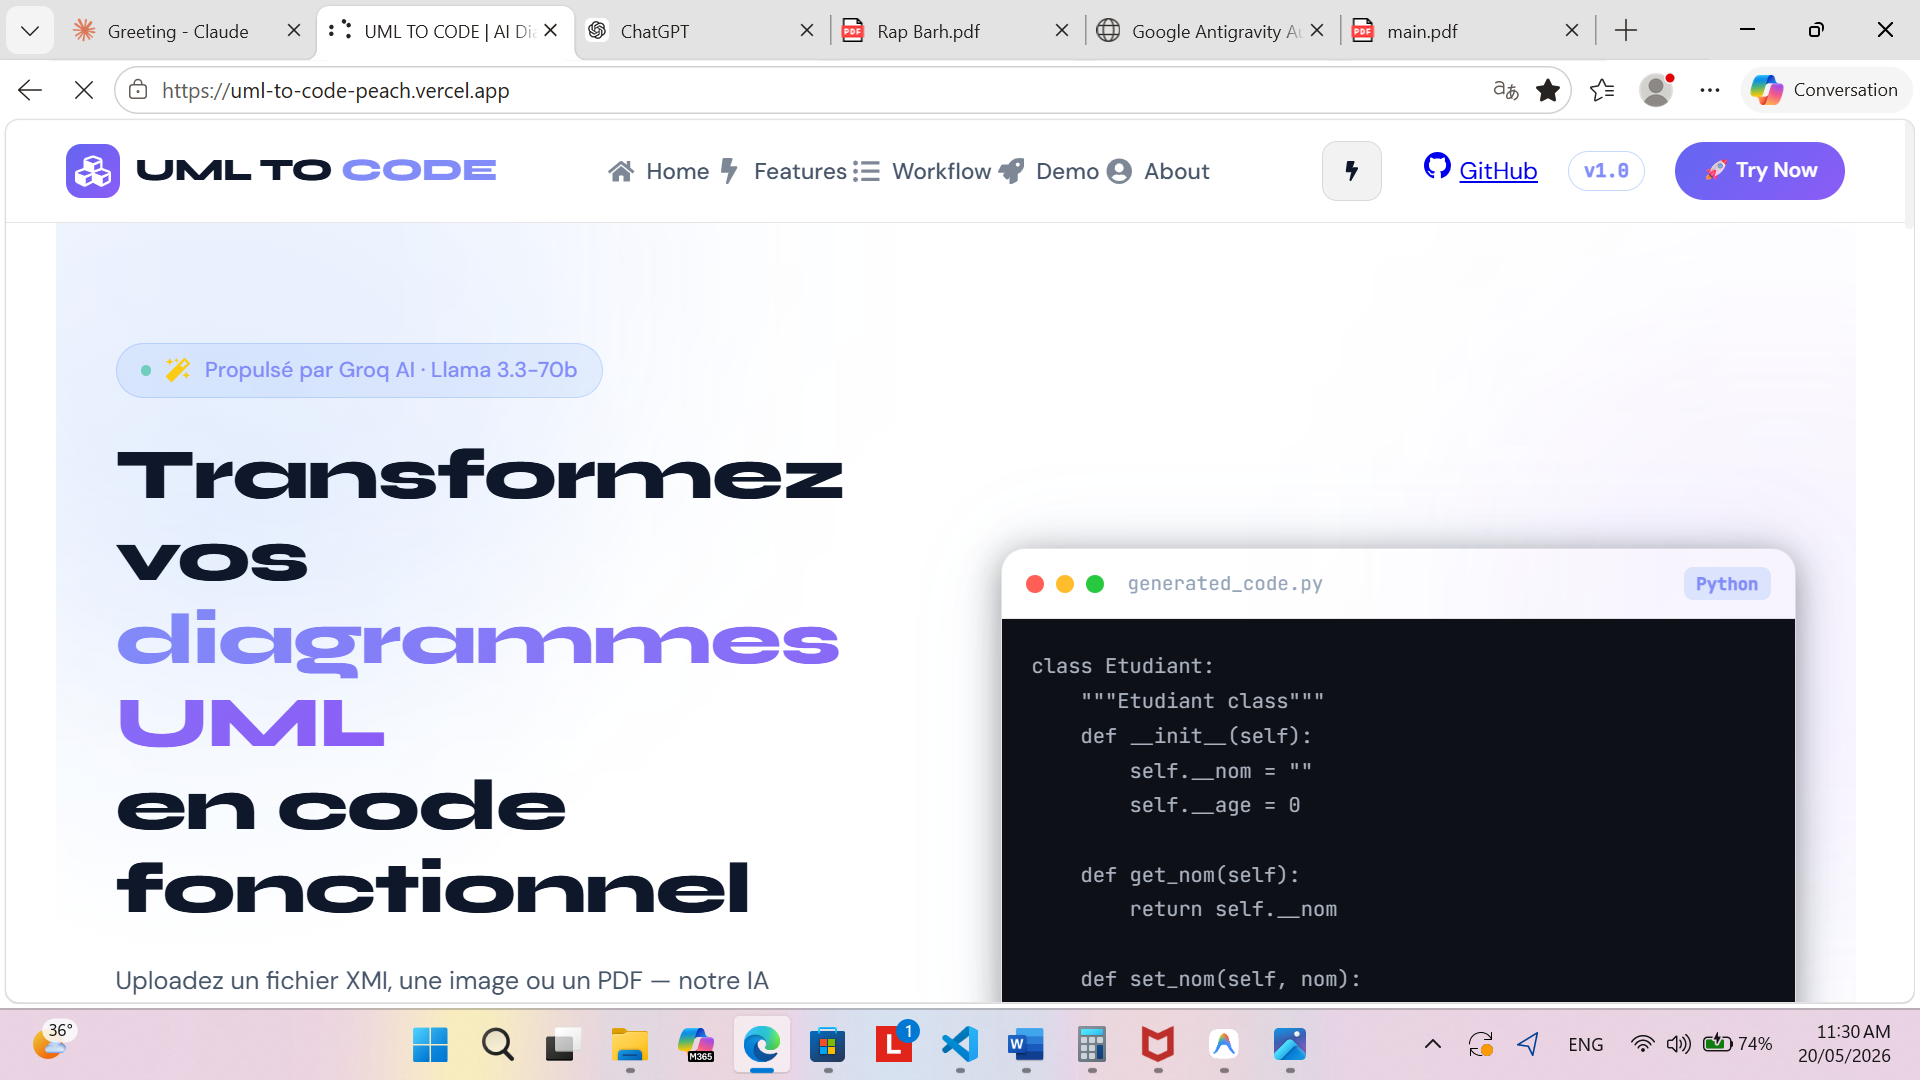
\includegraphics[width=\textwidth]{screenshots/hero.png}
    \caption{Page d'accueil — UML-to-Code (mode sombre)}
\end{figure}

\begin{figure}[H]
    \centering
    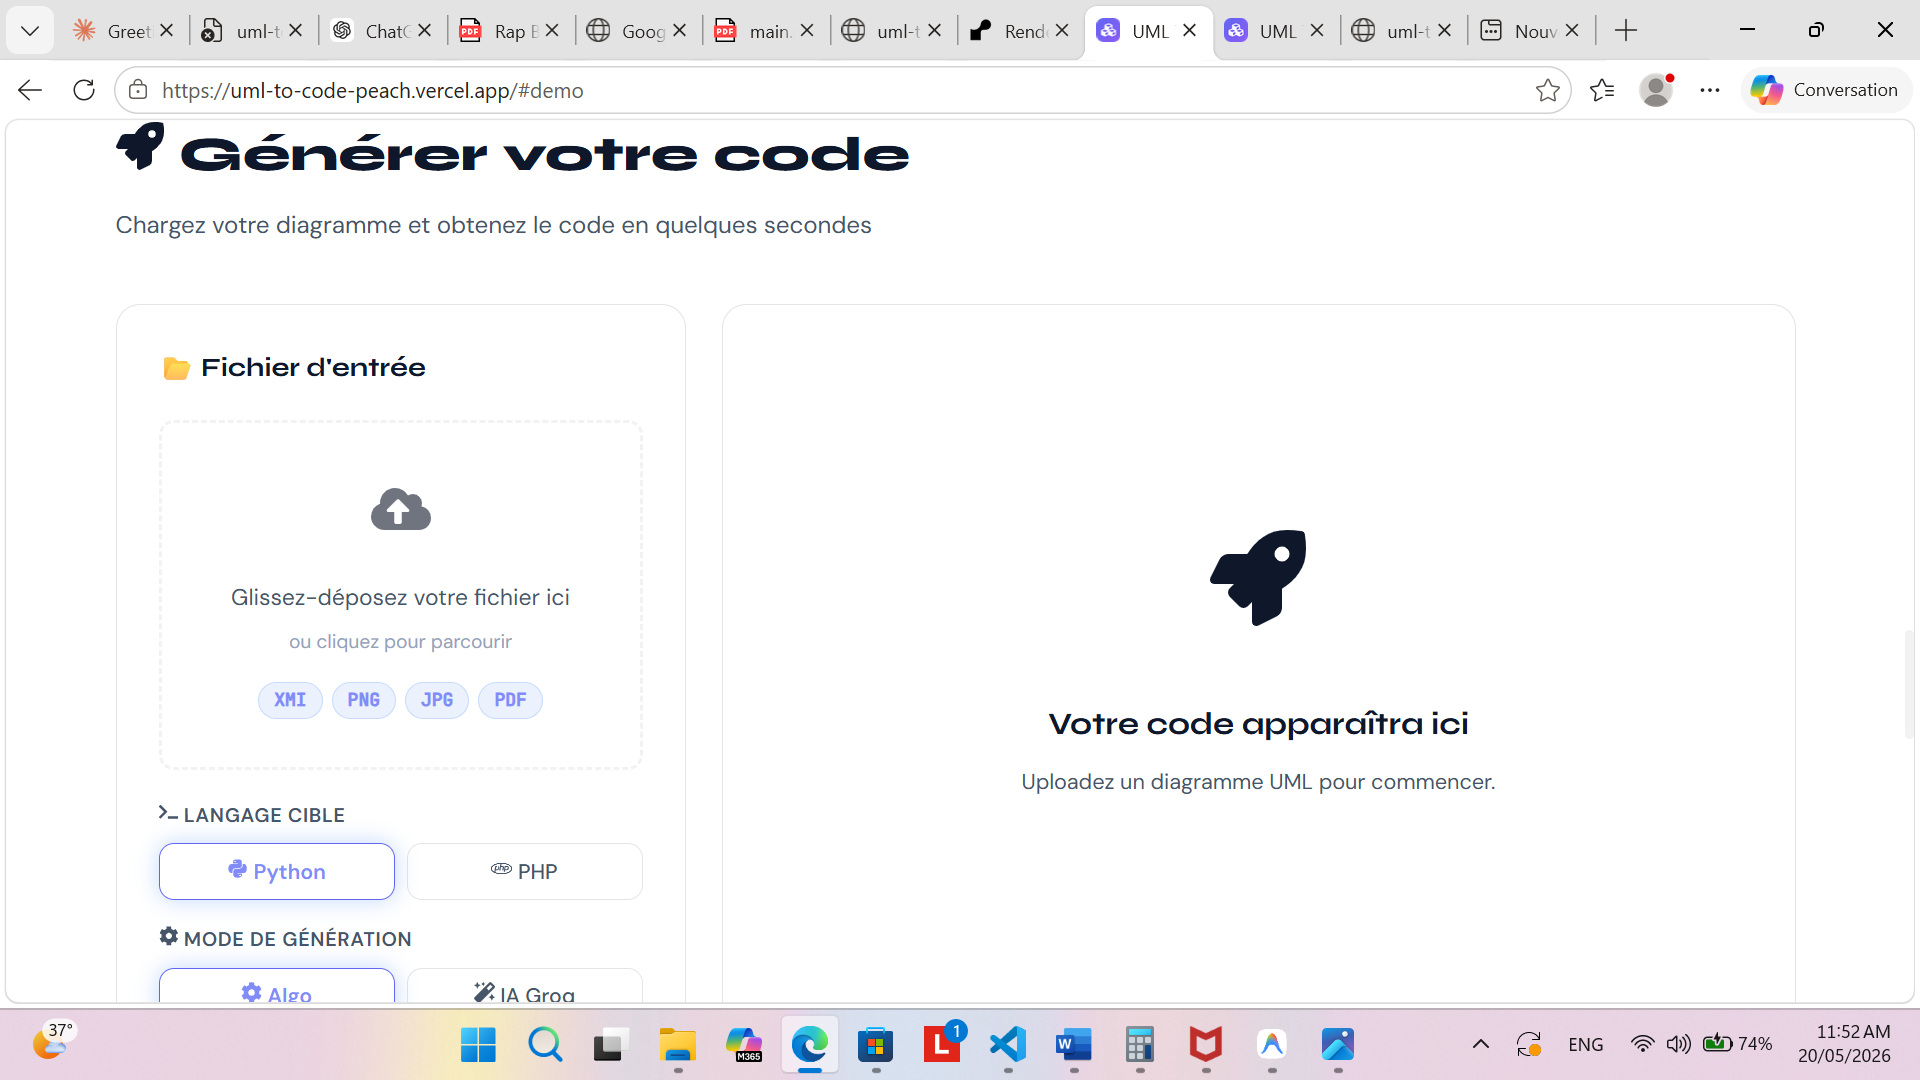
\includegraphics[width=\textwidth]{screenshots/demo.png}
    \caption{Zone de génération — Upload et Monaco Editor}
\end{figure}

\begin{figure}[H]
    \centering
    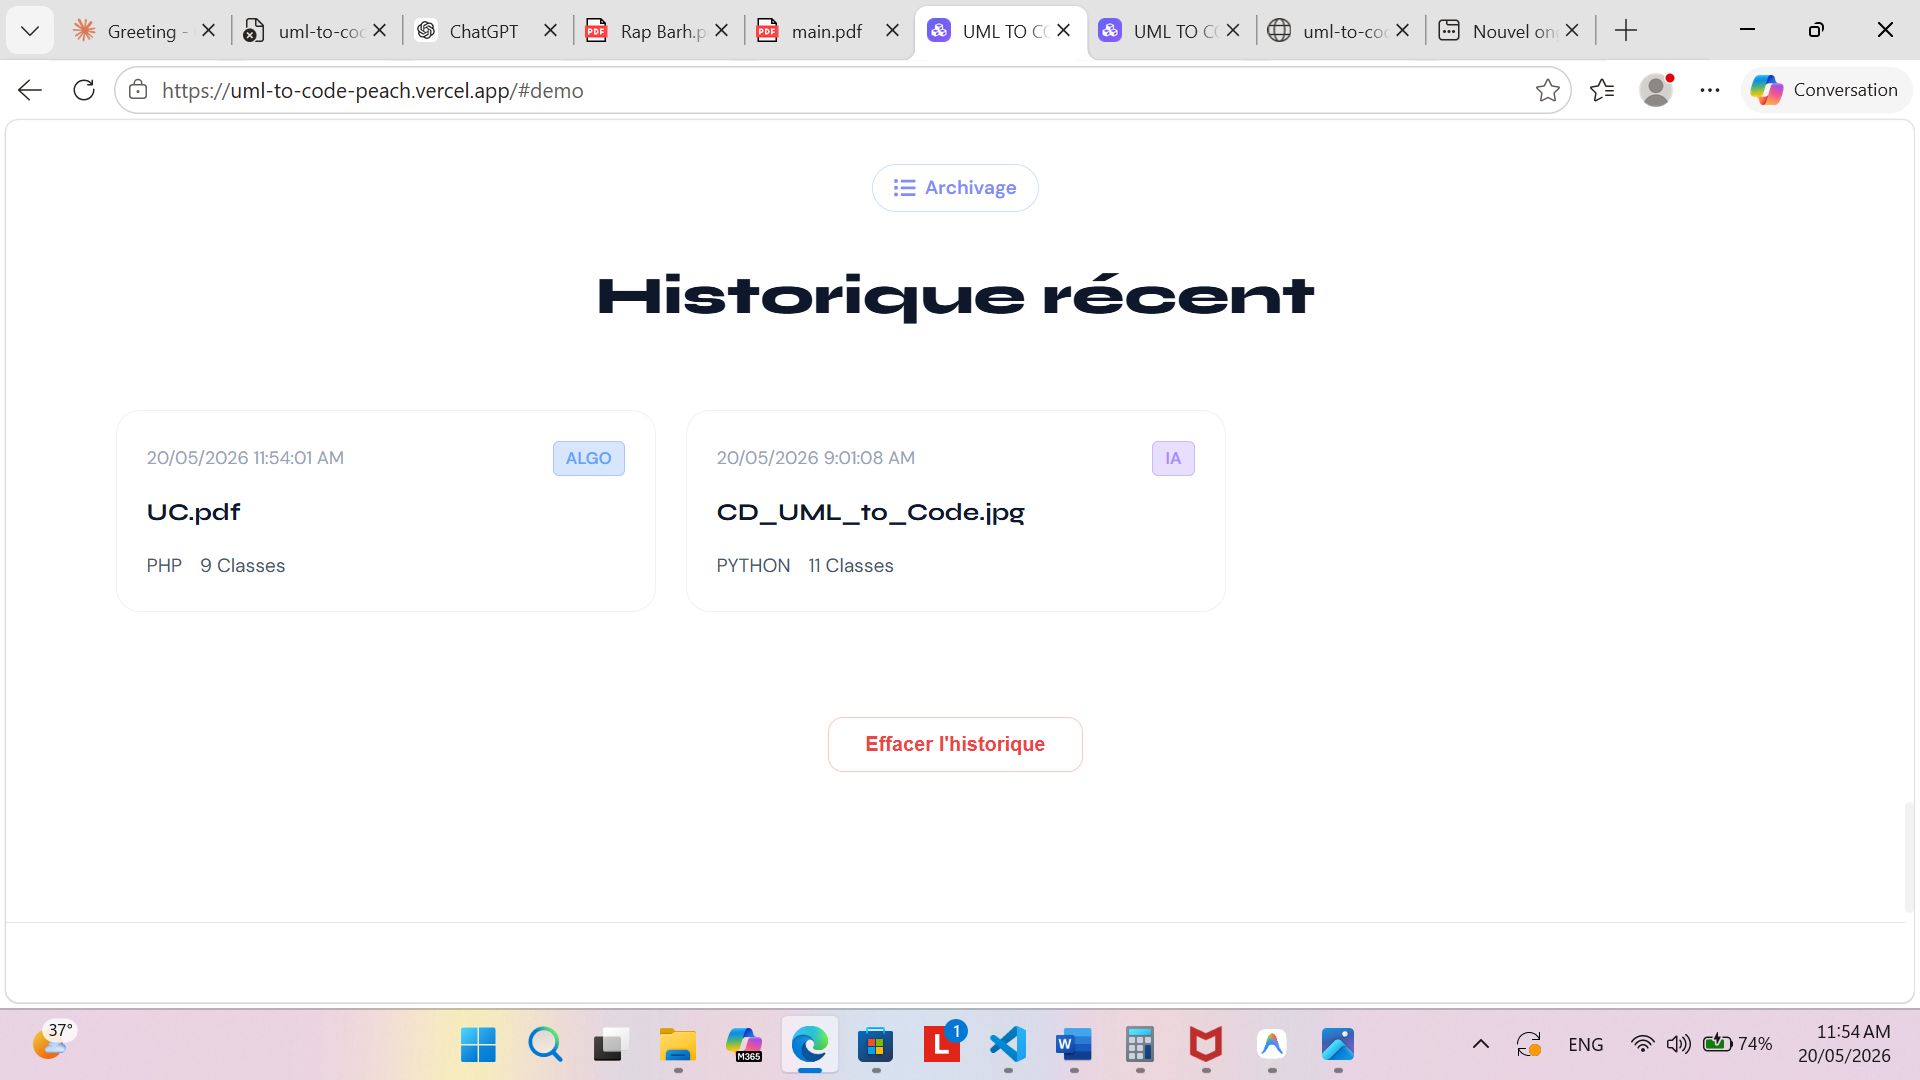
\includegraphics[width=\textwidth]{screenshots/history.png}
    \caption{Section Historique — 10 dernières générations}
\end{figure}

\chapter*{Conclusion Générale}
\addcontentsline{toc}{chapter}{Conclusion Générale}
\thispagestyle{plain}
\pagestyle{plain}
\markboth{}{}

La conception et la réalisation de la plateforme \textbf{UML-to-Code} ont constitué une expérience hautement enrichissante, marquant l'aboutissement de notre formation en Génie Logiciel à l'Institut National Supérieur des Sciences et Techniques d'Abéché (INSTA). Ce projet est né d'un constat simple mais critique dans l'industrie du logiciel : la nécessité de réduire le fossé temporel et technique entre la modélisation architecturale et l'implémentation concrète du code source.

Tout au long de ce document, nous avons démontré comment l'approche du Développement Dirigé par les Modèles (MDD) pouvait être matérialisée par un outil moderne et accessible. En partant de l'analyse des besoins jusqu'au déploiement de l'architecture client-serveur, le projet a suivi un cycle de vie incrémental rigoureux, permettant de valider chaque composant technologique.

Les résultats obtenus sont très satisfaisants et répondent intégralement aux objectifs fixés. La plateforme réussit le pari d'offrir :
\begin{itemize}
    \item Une robustesse absolue via son moteur de parsing XML (\texttt{xml.etree}) capable d'extraire la sémantique précise des fichiers XMI normalisés par l'OMG.
    \item Une flexibilité sans précédent grâce à l'intégration de l'Intelligence Artificielle (Llama 3.3), qui brise les barrières des formats d'exportation propriétaires en permettant la génération de code à partir de simples images ou PDF de diagrammes.
    \item Un confort d'utilisation professionnel, matérialisé par une interface "Glassmorphism" épurée intégrant l'éditeur de code Monaco, véritable standard de l'industrie.
\end{itemize}

Sur le plan personnel, ce projet de fin d'études a été un formidable terrain d'application pour consolider mes acquis. Il a exigé une maîtrise complète de la pile technologique "Full-Stack" (React.js, Flask, Python), une compréhension profonde des standards d'architecture logicielle (UML, XML/XMI), ainsi qu'une capacité à appréhender et intégrer les technologies émergentes (LLM via API).

\section*{Perspectives d'évolution}
Bien que fonctionnelle et aboutie, l'application \textbf{UML-to-Code} constitue une fondation sur laquelle de nombreuses évolutions peuvent être envisagées pour en faire un outil de qualité industrielle :
\begin{itemize}
    \item \textbf{Extension sémantique} : Prendre en charge d'autres types de diagrammes UML (Diagrammes de Séquence pour générer le corps des fonctions, Diagrammes d'États-Transitions pour générer des machines à états).
    \item \textbf{Diversification linguistique} : Ajouter des générateurs pour d'autres langages fortement typés tels que Java, C++, ou TypeScript, ainsi que la prise en charge de frameworks ORM (comme SQLAlchemy ou Doctrine).
    \item \textbf{Intégration au flux de travail (CI/CD)} : Développer la solution sous forme d'extension native pour des IDE (Visual Studio Code, IntelliJ) afin que la génération se fasse de manière transparente durant le développement.
\end{itemize}

En définitive, \textbf{UML-to-Code} illustre parfaitement comment l'alliance entre les méthodes classiques d'ingénierie logicielle et les avancées fulgurantes de l'intelligence artificielle peut redéfinir et optimiser le métier de développeur pour les années à venir.
\newpage


\bibliographystyle{plain}
\bibliography{references}

\chapter*{Webographie}
\addcontentsline{toc}{chapter}{Webographie}
\markboth{Webographie}{Webographie}

\vspace*{0.5cm}

\begin{enumerate}

\item \textbf{Groq — Documentation officielle de l'API}\\
Documentation complète de l'API Groq et du modèle Llama 3.3-70b.\\
\url{https://console.groq.com/docs}\\
\textit{Consulté en mai 2026}

\item \textbf{React.js — Documentation officielle}\\
Guide complet de React.js pour la création d'interfaces utilisateur.\\
\url{https://react.dev}\\
\textit{Consulté en mai 2026}

\item \textbf{Flask — Documentation officielle}\\
Documentation du micro-framework web Python Flask.\\
\url{https://flask.palletsprojects.com}\\
\textit{Consulté en mai 2026}

\item \textbf{Monaco Editor — Documentation}\\
Documentation de l'éditeur de code Monaco (moteur de VS Code).\\
\url{https://microsoft.github.io/monaco-editor}\\
\textit{Consulté en mai 2026}

\item \textbf{StarUML — Documentation officielle}\\
Guide d'utilisation de StarUML et export XMI.\\
\url{https://docs.staruml.io}\\
\textit{Consulté en mai 2026}

\item \textbf{Vercel — Documentation de déploiement}\\
Guide de déploiement d'applications React sur Vercel.\\
\url{https://vercel.com/docs}\\
\textit{Consulté en mai 2026}

\item \textbf{Render — Documentation de déploiement}\\
Guide de déploiement d'applications Python Flask sur Render.\\
\url{https://render.com/docs}\\
\textit{Consulté en mai 2026}

\item \textbf{PyMuPDF — Documentation officielle}\\
Documentation de la bibliothèque PyMuPDF pour le traitement de PDF.\\
\url{https://pymupdf.readthedocs.io}\\
\textit{Consulté en mai 2026}

\item \textbf{UML — Spécification OMG}\\
Spécification officielle du langage UML par l'Object Management Group.\\
\url{https://www.omg.org/spec/UML}\\
\textit{Consulté en mai 2026}

\item \textbf{XMI — Spécification OMG}\\
Spécification officielle du format XMI par l'Object Management Group.\\
\url{https://www.omg.org/spec/XMI}\\
\textit{Consulté en mai 2026}

\item \textbf{GitHub — Dépôt du projet UML-to-Code}\\
Code source complet du projet disponible en open source.\\
\url{https://github.com/ABAKAR5/uml-to-code}\\
\textit{Consulté en mai 2026}

\item \textbf{Application déployée — UML-to-Code}\\
Application web déployée et accessible en ligne.\\
\url{https://uml-to-code-peach.vercel.app}\\
\textit{Consulté en mai 2026}

\end{enumerate}

\clearpage
\pagestyle{empty}

\end{document}
